\newcommand{\Subject}{\textcolor{black}{NATO Workshop on Modelling and Simulation for Autonomous Systems}\\{---}\\\LARGE{Spatiotemporal models of human activity for robotic patrolling}}
\newcommand{\Meeting}{MESAS 2018, Prague}
\newcommand{\Author}{Tom{\'a}{\v s} Vintr}
\newcommand{\Authors}{Tom{\'a}{\v s} Vintr, Kerem Eyisoy, Vanda Vintrov{\'a}, Tom{\'a}{\v s} Krajn{\'i}k}
\newcommand{\Date}{}
%\usetheme{warsaw}

\newcommand{\video}[2]{\href{run:#1}{\includegraphics[width=0.99\textwidth]{#2}}}
\newcommand{\link}[2]{\href{run:#1}{\includegraphics[width=0.99\textwidth]{#2}}}
\newcommand{\bib}[3]{\begin{thebibliography}{#1}\bibitem[#1]{#1}{#2}.\newblock{\em #3}\end{thebibliography}}

\newcommand{\Lincoln}{Artificial Intelligence Center, Faculty of Electrical Engineering, Czech Technical University,\\Department of Computer Engineering, Faculty of Engineering, Marmara University,\\Faculty of Informatics and Statistics, University of Economics, Prague}
\newcommand{\Institute}{\Lincoln\\}


\newcommand{\HeadLineLeft}{Tom{\'a}{\v s} Vintr}
\newcommand{\HeadLineCenter}{NATO Workshop on Modelling and Simulation for Autonomous Systems}
\newcommand{\HeadLineRight}{AIC@CTU}
\newcommand{\FootLineCenter}{Spatiotemporal models of human activity for robotic patrolling}
\newcommand{\FootLineLeft}{\insertshortauthor}

% File name: head.tex
% Date:      2008/09/28 20:40
% Author:    Jan Faigl

\newread\testin
\def\softinput #1 {\let\next=\relax \openin\testin=#1
\ifeof\testin \message{Info: the file #1 does not exist}%
\else \closein\testin \def\next{\input #1 }\fi
\next}

\softinput{makeconfig}

\ifx\print\undefined
\documentclass[mathserif]{beamer}
% File name: head-beamer.tex
% Date:      2008/09/28 20:40
% Author:    Jan Faigl

%\usepackage[latin2]{inputenc}
%\usepackage{times}
\usepackage[T1]{fontenc}
\usepackage{helvet}
\usepackage{graphicx}
\usepackage{multimedia}
\usepackage{hyperref}
\usepackage{amsmath}
\usepackage{textcomp}

\usepackage{listings}
\usepackage{ragged2e}

\lstset{extendedchars=true}
\lstset{inputencoding=latin2}
\lstset{breaklines=true,basicstyle=\tiny,language=sh}
\lstset{language=java}
\lstset{columns=fullflexible}
\definecolor{background_color}{gray}{0.9}
\definecolor{comment_color}{rgb}{0.0, 0.5, 0.0}
\definecolor{keyword_color}{rgb}{0.0, 0.0, 1.0}
\definecolor{string_color}{rgb}{0.8, 0.0, 0.0}

\lstset{keywordstyle=\color{keyword_color}\bfseries}
\lstset{commentstyle=\color{comment_color}}
\lstset{stringstyle=\color{string_color}}
\lstset{basicstyle=\ttfamily}
\lstset{showstringspaces=false}
\lstset{keepspaces=true}
\lstset{tabsize=2}
\lstset{breaklines=true}

\institute{\Institute}

\date{\Date}
\author[\Author]{\Authors}
\newcommand{\disable}[1]{}

\colorlet{redshaded}{red!25!bg}
\colorlet{shaded}{black!25!bg}
\colorlet{shadedshaded}{black!10!bg}
\colorlet{blackshaded}{black!40!bg}

\colorlet{darkred}{red!80!black}
\colorlet{darkblue}{blue!80!black}
\colorlet{darkgreen}{green!80!black}

\newcommand{\myurl}[1]{{\color{blue}\url{#1}}}

\DeclareMathOperator{\argmax}{argmax}

\pgfdeclareimage[height=0.4cm]{GL}{fig/gl-logo}
\pgfdeclareimage[height=1.0cm]{logoGL}{fig/logoGL}
%\logo{\pgfuseimage{GL}}
\logo{\pgfuseimage{logoGL}}

\usetheme{Singapore}

\setbeamercovered{transparent}
\setbeamertemplate{navigation symbols}{ }

\defbeamertemplate*{part page}{}[1][]{
\begin{centering}
   {\usebeamerfont{part name}\usebeamercolor[fg]{part name}Part~\insertromanpartnumber}
   \vskip1em\par
   \begin{beamercolorbox}[sep=8pt,center,#1]{part title}
      \usebeamerfont{part title}\insertpart\par
   \end{beamercolorbox}
\end{centering}
}        

\setbeamerfont{code}{size={\fontsize{11pt}{6pt}}}
\setbeamerfont{codeSmall}{size={\fontsize{10pt}{6pt}}}
\setbeamerfont{codeSmaller}{size={\fontsize{9pt}{6pt}}}
\setbeamerfont{small}{size={\fontsize{8pt}{6pt}}}
\AtBeginPart{\frame{\partpage}}


\setbeamercolor{alerted text}{fg=red!80!black}

%-----------------------------------------------------------------------------
% Header line
%-----------------------------------------------------------------------------

\defbeamertemplate*{headline}{}
{%
\begin{beamercolorbox}[colsep=1.5pt]{upper separation line head}
\end{beamercolorbox}
\hbox{%
\begin{beamercolorbox}[wd=0.15\paperwidth,ht=2.25ex,dp=1ex,left]{section in head/foot}%
   \usebeamerfont{title in head/foot}\hspace*{2ex}\HeadLineLeft\hspace*{2ex}
\end{beamercolorbox}%
\begin{beamercolorbox}[wd=0.7\paperwidth,ht=2.25ex,dp=1ex,center]{subsection in head/foot}%
  \usebeamerfont{subsection in head/foot}\hspace*{2ex}\HeadLineCenter
\end{beamercolorbox}%
\begin{beamercolorbox}[wd=0.15\paperwidth,ht=2.25ex,dp=1ex,left]{section in head/foot}%
   \usebeamerfont{section in head/foot}\hspace*{1ex}\HeadLineRight
\end{beamercolorbox}%
}
%\begin{beamercolorbox}{section in head/foot}
%   \vskip2pt\insertsectionnavigationhorizontal{\paperwidth}{}{}\vskip2pt
% \end{beamercolorbox}%

\begin{beamercolorbox}[colsep=1.5pt]{lower separation line head}
\end{beamercolorbox}
}
\addtoheadtemplate{\pgfuseshading{beamer@headfade}\vskip-1.25cm}{}

%-----------------------------------------------------------------------------
% footline
%-----------------------------------------------------------------------------
\defbeamertemplate*{footline}{}{
\leavevmode%
\hbox{%
\begin{beamercolorbox}[wd=.22\paperwidth,ht=2.25ex,dp=1ex,left]{author in head/foot}%
   \usebeamerfont{author in head/foot}\hspace*{2ex}\FootLineLeft\hspace*{2ex}
\end{beamercolorbox}%
\begin{beamercolorbox}[wd=.68\paperwidth,ht=2.25ex,dp=1ex,center]{institute in head/foot}%
   \usebeamerfont{title in head/foot}\FootLineCenter
\end{beamercolorbox}%
\begin{beamercolorbox}[wd=0.1\paperwidth,ht=2.25ex,dp=1ex,right]{date in head/foot}%
   \insertframenumber{} / \inserttotalframenumber\hspace*{1ex}
\end{beamercolorbox}}%
\vskip0pt%
}

\else
\documentclass[trans]{beamer}
% File name: head-print.tex
% Date:      2008/09/28 20:40
% Author:    Jan Faigl

\usepackage[latin2]{inputenc}
\usepackage{times}
\usepackage[T1]{fontenc}
\usepackage{helvet}
\usepackage{graphicx}
\usepackage{multimedia}
\usepackage{hyperref}
\usepackage{amsmath}
\usepackage{textcomp}

\usepackage{listings}
\usepackage{ragged2e}

\lstset{extendedchars=true}
\lstset{inputencoding=latin2}
\lstset{breaklines=true,basicstyle=\tiny,language=sh}
\lstset{language=java}
\lstset{columns=fullflexible}
\definecolor{background_color}{gray}{0.9}
\definecolor{comment_color}{rgb}{0.0, 0.5, 0.0}
\definecolor{keyword_color}{rgb}{0.0, 0.0, 1.0}
\definecolor{string_color}{rgb}{0.8, 0.0, 0.0}

\lstset{keywordstyle=\color{keyword_color}\bfseries}
\lstset{commentstyle=\color{comment_color}}
\lstset{stringstyle=\color{string_color}}
\lstset{basicstyle=\ttfamily}
\lstset{showstringspaces=false}
\lstset{keepspaces=true}
\lstset{tabsize=2}
\lstset{breaklines=true}

\institute{\Institute}

\date{\Date}
\author[\Author]{\Subject}
\newcommand{\disable}[1]{}

\colorlet{redshaded}{red!25!bg}
\colorlet{shaded}{black!25!bg}
\colorlet{shadedshaded}{black!10!bg}
\colorlet{blackshaded}{black!40!bg}

\colorlet{darkred}{red!80!black}
\colorlet{darkblue}{blue!80!black}
\colorlet{darkgreen}{green!80!black}

\newcommand{\myurl}[1]{{\color{blue}\url{#1}}}

\DeclareMathOperator{\argmax}{argmax}

\pgfdeclareimage[height=0.4cm]{GL}{fig/gl-logo}
\pgfdeclareimage[height=0.4cm]{logoGL}{fig/logoGL}
\logo{\pgfuseimage{GL}}
%\logo{\pgfuseimage{logoGL}}

\usetheme{default}

\setbeamercovered{transparent}
\setbeamertemplate{navigation symbols}{ }

\defbeamertemplate*{part page}{}[1][]{
\begin{centering}
   {\usebeamerfont{part name}\usebeamercolor[fg]{part name}��st~\insertromanpartnumber}
   \vskip1em\par
   \begin{beamercolorbox}[sep=8pt,center,#1]{part title}
      \usebeamerfont{part title}\insertpart\par
   \end{beamercolorbox}
\end{centering}
}        

\setbeamerfont{code}{size={\fontsize{11pt}{6pt}}}
\setbeamerfont{codeSmall}{size={\fontsize{10pt}{6pt}}}
\setbeamerfont{codeSmaller}{size={\fontsize{9pt}{6pt}}}
\setbeamerfont{small}{size={\fontsize{8pt}{6pt}}}
\AtBeginPart{\frame{\partpage}}


\setbeamercolor{alerted text}{fg=red!80!black}


%-----------------------------------------------------------------------------
% footline
%-----------------------------------------------------------------------------
\defbeamertemplate*{footlineX}{}{
\leavevmode%
\hbox{%
\begin{beamercolorbox}[wd=.34\paperwidth,ht=2.25ex,dp=1ex,left]{author in head/foot}%
   \usebeamerfont{author in head/foot}\hspace*{2ex}\FootLineLeft\hspace*{2ex}
\end{beamercolorbox}%
\begin{beamercolorbox}[wd=.51\paperwidth,ht=2.25ex,dp=1ex,center]{institute in head/foot}%
   \usebeamerfont{title in head/foot}\FootLineCenter
\end{beamercolorbox}%
\begin{beamercolorbox}[wd=0.14\paperwidth,ht=2.25ex,dp=1ex,right]{date in head/foot}%
   \insertframenumber{} / \inserttotalframenumber\hspace*{1ex}
\end{beamercolorbox}}%
\vskip0pt%
}

\fi


\title{{\bf \Subject}}
\usepackage{multirow}
\begin{document}
% - frame ---------------------------------------------------------------------

\frame{\titlepage}

\begin{frame}
	\frametitle{Self Learning Autonomous System for Patrolling}
    \vspace{3mm}
    \href{run:./video/Linda patrolling MHT office-_tXOevb51rc.mp4}{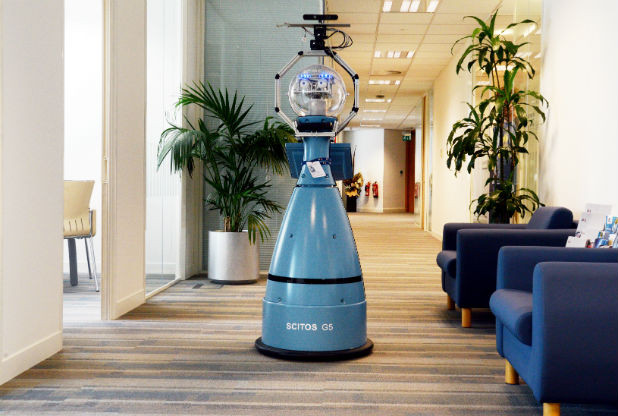
\includegraphics[width=0.9\textwidth]{fig/The-robot-Linda-at-Open-space-office-and-Bob-at-office-corridor.png}}
%    \centering\video{cmds/uvodni_video.sh}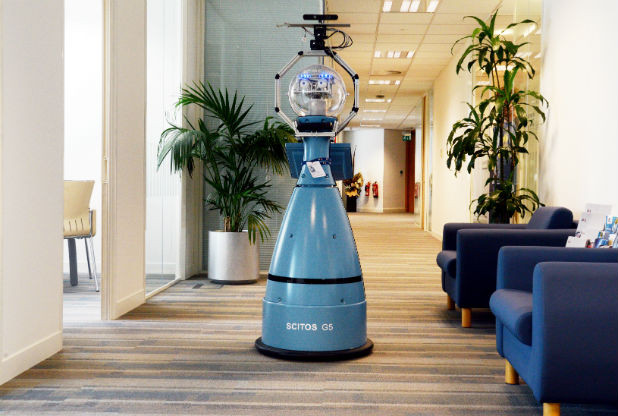
\includegraphics[width=0.7\textwidth]{fig/The-robot-Linda-at-Open-space-office-and-Bob-at-office-corridor.png}
	\begin{center}
	Towards the ability to understand an human-populated environment.
	\end{center}
\end{frame}







% - frame --------------------------------------------------------------------
\begin{frame}
   \frametitle{Detection of an Anomalous Behavior}
    \vspace{3mm}
	\begin{columns}
	%\hfill
	        \column{0.45\textwidth}
    \only<1,2,3>{
	            Standard solution:
                \begin{enumerate}
                   \item  Define rules,
                   \item  hard-code rules,
                   \item  update rules regularly.
                \end{enumerate}
        }
	        \column{0.45\textwidth}
    \only<1,2,3>{
        \invisible<1>{
	            Problems:
                \begin{enumerate}
	                \item  Expert opinion,
	                \item  different scenarios,
	                \item  keep software updated.
                \end{enumerate}
        }
    }
   \end{columns}
%
    \only<1,2,3>{
        \invisible<1>{
            \centering
            \includegraphics[width=0.7\textwidth]{fig/become-a-programmer.jpg}
        }
    }

    \only<1,2,3>
        {\invisible<1,2>{
            \begin{center}
	            To overcome the aforementioned problems,\\we propose \textbf{self learning} autonomous system.
            \end{center}
         }
    }
\end{frame}


\section{Method}
% - frame ---------------------------------------------------------------------
\begin{frame}
   \frametitle{Suitable Tools to Model Human Habits}
        %\item Hist24 - histogram of occurences during day,
        %\item Hist168 - histogram of occurences during week,
        %\item Prophet - SOTA in time series forcasting,
        %\item FreMEn - SOTA in long-term autonomy,
    \vspace{3mm}
    \only<1,2,3,4>{
        \invisible<1>{
            \centerline{\href{run:./video/pitch.mkv}{\textbf{FreMEn}} - Frequency Map Enhancement}
            \begin{itemize}
                \item State of the Art in Long-Term Robotics,
                \item can detect and model multiple periodicities in measured phenomenon,
	            \item successfully deployed in autonomous robot patrolling,
                \item not meant as a tool to search for outliers.
            \end{itemize}
    \vspace{3mm}
        }
    }
    \only<1,2,3, 4>{
        \invisible<1,2>{
            \centerline{\textbf{Hist24} and \textbf{Hist168} - histograms of occurences}
            \begin{itemize}
                \item Histograms over one day, resp. one week,
                \item favourite (simple) solution in long-term robotics,
                \item describe only one predefined periodicity of measured phenomenon.
            \end{itemize}
            %\vspace{3mm}
        }
    }
    \only<1,2,3,4>{
        \invisible<1,2,3>{
            \centerline{\textbf{Prophet}}
            \begin{itemize}
	            \item User friendly tool for time series forcasting from Facebook,
                \item designed for economic time series.
            \end{itemize}
            %\vspace{3mm}
        }
    }
%\href{run:./video/pitch.mkv}{Click for video}
\end{frame}


%\renewcommand{\Author}{Krajnik, Faigl, Vonasek et al.: }
%\renewcommand{\FootLineCenter}{\textbf{Simple, Yet Stable Bearing only Navigation}. Journal of Field Robotics, 2010}
% - frame ---------------------------------------------------------------------
\begin{frame}
   \frametitle{Our Solution to Model Human Habits}
    %\vspace{3mm}
    \begin{itemize}
    \only<1,2,3,4>{
        \invisible<1>{
            \item Use FreMEn to detect periodicities in human behavior,
        }
    }
    %\vspace{5mm}
    \only<1,2,3,4>{
        \invisible<1,2>{
            \item project timeseries into \textbf{\textcolor{darkred}{\textcolor{red}{W}arped \textcolor{red}{Hy}per\textcolor{red}{T}im\textcolor{red}{e}}},

%\hfill
        }
    }
    \only<1,2,3,4>{
        \invisible<1,2,3>{
            \item and model phenomenons using Gaussian mixtures.
        }
    }

    \end{itemize}
    \vspace{3mm}
    \only<1>{
        \invisible<1>{
            \includegraphics[width=1.0\textwidth]{fig/hypertime_graph_v2.pdf}
        }
    }
    \only<2>{
            \includegraphics[width=1.0\textwidth]{fig/hypertime_graph_1.pdf}
    }
    \only<3>{
            \includegraphics[width=1.0\textwidth]{fig/hypertime_graph_2.pdf}
    }
    \only<4>{
            \includegraphics[width=1.0\textwidth]{fig/hypertime_graph_3.pdf}
    }
\end{frame}




% - frame ---------------------------------------------------------------------
\begin{frame}
   \frametitle{Outlier Detection}
    \vspace{3mm}
    \centerline{Outliers:}
    \begin{itemize}
        \item Vaguely defined,
        \item unexpected, inconsistent, suspicious, or rare measurements.
    \end{itemize}
    \only<1,2,3>{
        \invisible<1>{
    \centerline{Outlier Hypothesis:}
	\begin{columns}
	    \column{0.45\textwidth}
                \begin{itemize}
                   \item  Detection:
                   \item  Model:
                   \item  Significance level:
                \end{itemize}
	        \column{0.45\textwidth}
                \begin{itemize}
	                \item  model based.
	                \item  Bernoulli distribution.
	                \item  $\alpha = 0.1.$%,$ $\alpha = 0.01.$
                \end{itemize}
   \end{columns}
        }
    }
    \vspace{5mm}
   \only<1,2,3>{
        \invisible<1,2>{
    \centerline{Measure to Compare Methods:}
    \begin{itemize}
        \item Matthews correlation coefficient ( <-1; 1> ).
    \end{itemize}
        }
    }

\end{frame}



% - frame ---------------------------------------------------------------------
\begin{frame}
   \frametitle{Experiment Design and Data}
    \begin{itemize}
        \item Real world dataset (Lincoln University office),
        \item twenty weeks of person detection (detected or not),
        \item training datasets: first day to first three weeks,
        \item test dataset: eighteenth week,
        \item manually labeled anomalies in test data.
        \item methods to compare: Hist24, Hist168, Prophet, FreMEn, WHyTe.
       \end{itemize}
%     \centerline{Methods to Compare:}
%    \begin{itemize}
%        \item Hist24 - histogram of occurences during day,
%        \item Hist168 - histogram of occurences during week,
%        \item Prophet - SOTA in time series forcasting,
%        \item FreMEn - SOTA in long-term autonomy,
%        \item WHyTe - proposed method.
%    \end{itemize}

\hfill\includegraphics[width=0.48\textwidth]{fig/3_weeks.pdf}\hfill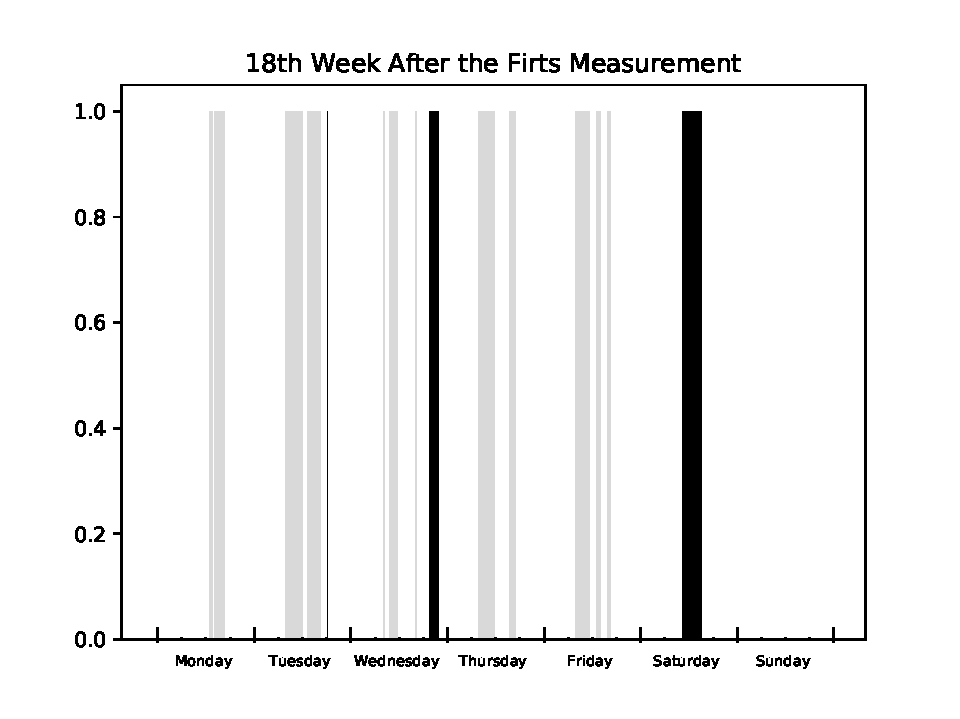
\includegraphics[width=0.48\textwidth]{fig/outliers_test.pdf}\hfill


\end{frame}



% - frame ---------------------------------------------------------------------
\begin{frame}
   \frametitle{Results, $\alpha = 0.1$}
    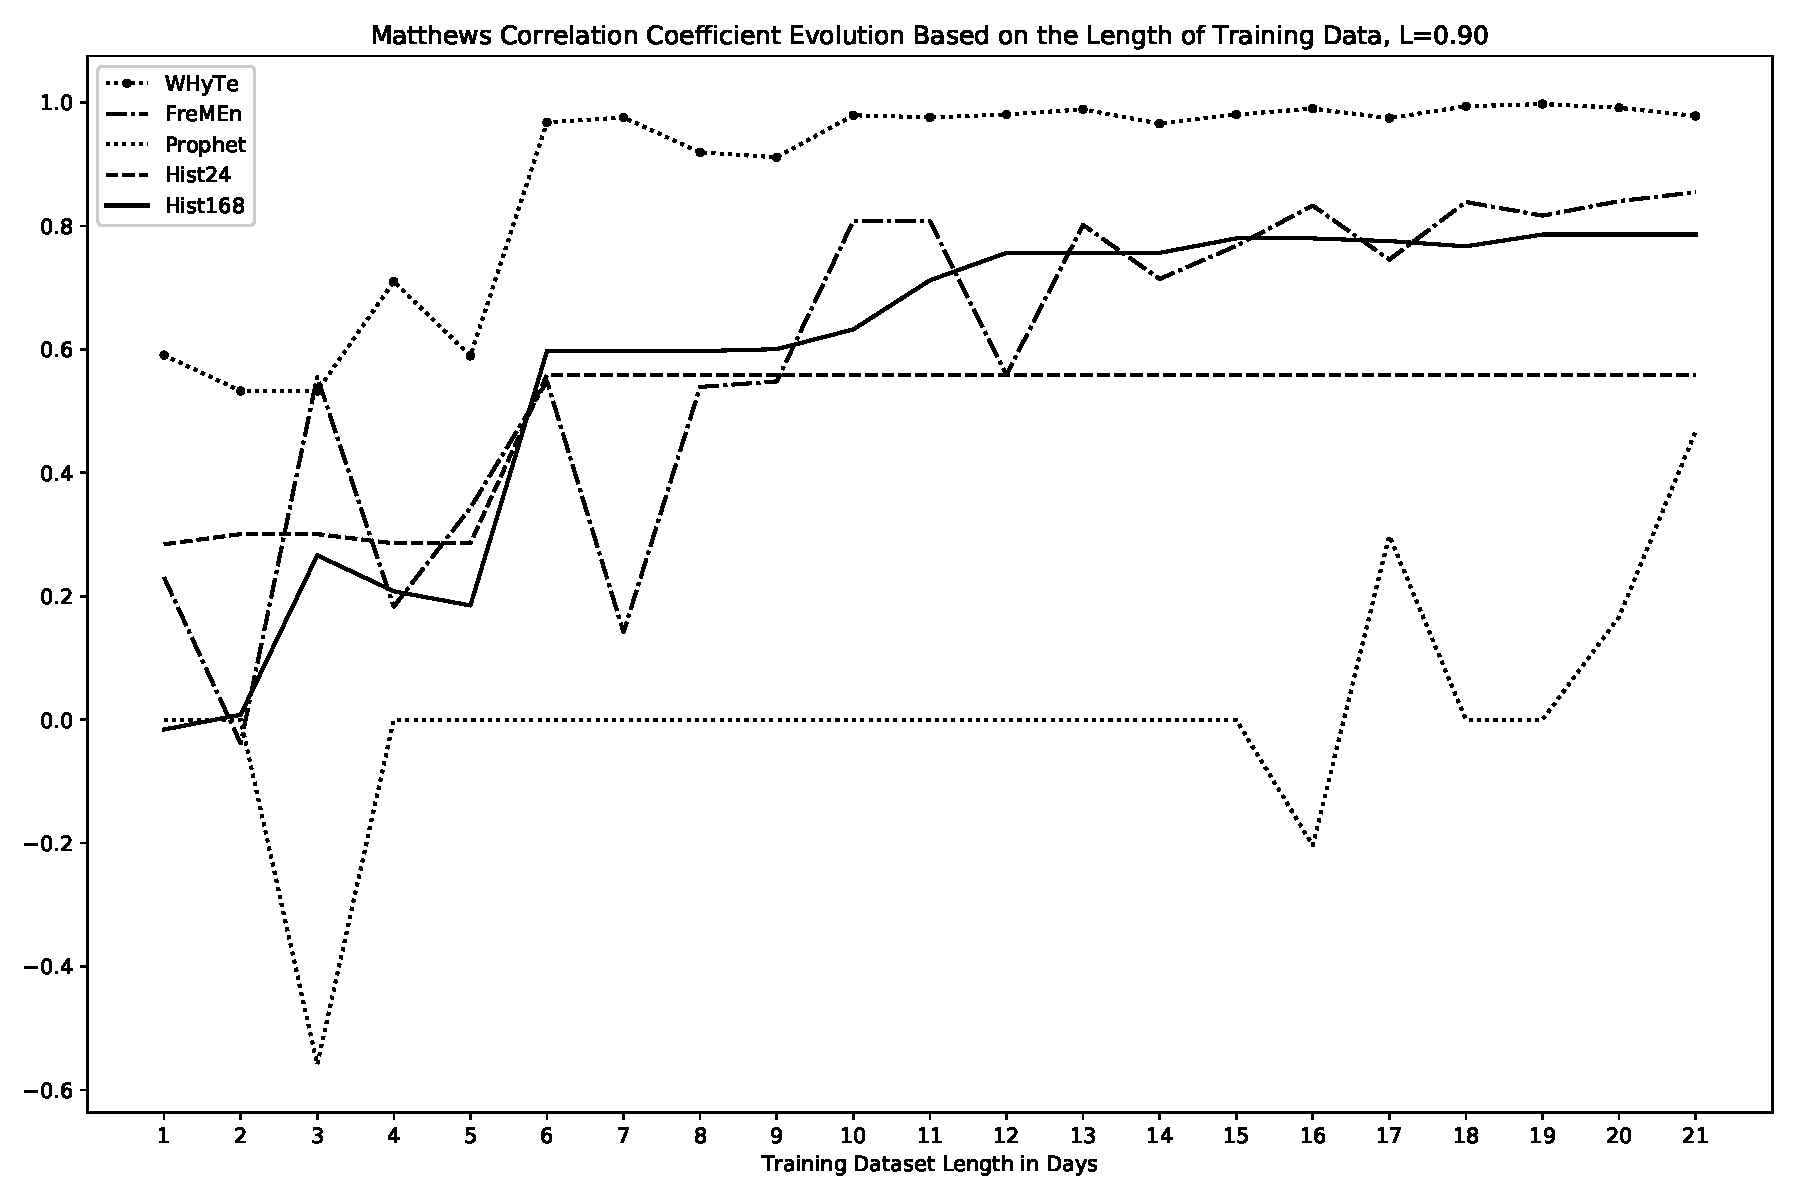
\includegraphics[width=1.0\textwidth]{fig/mathew_graph_90.pdf}
\end{frame}


% - frame ---------------------------------------------------------------------
%\begin{frame}
%   \frametitle{Results, $\alpha = 0.01$}
%    \includegraphics[width=1.0\textwidth]{fig/mathew_graph_99.pdf}
%\end{frame}



% - frame ---------------------------------------------------------------------
\begin{frame}
   \frametitle{Conclusion}
    \only<1,2,3>{
    \centerline{Improvement Proposal:}
    \begin{itemize}
        \item The self learning autonomous system to detect anomalous behaviour of humans in their natural environment.
    \end{itemize}
    }
    \only<1,2,3>{
        \invisible<1>{
    \centerline{Novelty:}
    \begin{itemize}
        \item The projection of time series into \textbf{warped hypertime}.
    \end{itemize}
        }
    }
    \only<1,2,3>{
        \invisible<1,2>{
    \centerline{Qualities:}
    \begin{itemize}
        \item Short time to learn,
        \item long time stability of forecasting,
        %\item robustness to the significance level choice,
        %\item reflects innate seassonality and continuity,
        \item uses usual statistical procedure and methods,
        \item outperforms State of the Art methods.
    \end{itemize}
        }
    }
\end{frame}



% - frame ---------------------------------------------------------------------
\begin{frame}
   \frametitle{Future Work}
		\vfill
    \begin{itemize}
        \item Generalize the method to analyze multidimensional data,
        \item evaluate the method to different scenarios.
		\vfill
    \end{itemize}
    \includegraphics[width=1.0\textwidth]{fig/all.png}
		\vfill
\end{frame}



% - frame ---------------------------------------------------------------------
\begin{frame}
	\frametitle{Questions}
	\begin{center}
		%\vfill
		%Code, paper and data available: \textbf{bearnav.eu}
		\vfill
		Thank you for your attention.\\
		\vfill
		Questions?
		\vfill
	\end{center}
\end{frame}


\end{document}
